\chapter{Conclusioni}
\label{cap:conclusioni}

\intro{In questo ultimo capitolo verranno illustrati gli obiettivi raggiunti, il consuntivo delle attività e infine verrà fornita una valutazione personale sul tirocinio svolto.}\\

\section{Obiettivi raggiunti}
\label{sec:raggiungimento-obiettivi}

La Tabella \ref{tab:obbiettivi-raggiunti} illustra gli obiettivi raggiunti al termine del tirocinio.

\begin{table}
    \centering
    \begin{tabularx}{\textwidth}{|c|X|c|c|}
        \hline
        \textbf{Obiettivo} & \textbf{Descrizione} & \textbf{Priorità} & \textbf{Stato} \\ \hline
        \hyperref[O01]{O01} & 
        Implementazione di meccanismi di autenticazione &
        Obbligatorio & 
        Soddisfatto \\ \hline
        \hyperref[O02]{O02} & 
        Richiamare i dati dal backend e visualizzarli all'interno dell'applicazione &
        Obbligatorio & 
        Soddisfatto \\ \hline
        \hyperref[O03]{O03} & 
        Implementazione di funzionalità per la creazione delle \textit{Meeting Note} &
        Obbligatorio & 
        Soddisfatto \\ \hline
        \hyperref[O04]{O04} & 
        Implementazione di funzionalità per la compilazione delle \textit{Meeting Note} &
        Obbligatorio & 
        Soddisfatto \\ \hline
        \hyperref[O05]{O05} & 
        Sviluppo interfaccia grafica dell'applicazione &
        Obbligatorio & 
        Soddisfatto \\ \hline
        \hyperref[D01]{D01} & 
        Integrazione del servizio OpenAI per automatizzare la creazione di \textit{Meeting Note} &
        Desiderabile & 
        Soddisfatto \\ \hline
        \hyperref[D02]{D02} & 
        Deploy dell'applicazione &
        Desiderabile & 
        Non soddisfatto \\ \hline
        \hyperref[F01]{F01} & 
        Esecuzione dei test per la verifica e validazione dell'applicazione &
        Facoltativo & 
        Non soddisfatto \\ \hline
    \end{tabularx}%
\caption{Tabella con gli obiettivi raggiunti}
\label{tab:obbiettivi-raggiunti}
\end{table}

\noindent Il mancato soddisfascimento degli obiettivi \emph{D02} e \emph{F01}, ovvero il \emph{deploy} e la stesura dei test per la verifica e validazione dell'applicazione, è stato causato principalmente dalla mancanza di tempo. \\
Come evidenziato dal reale svolgimento delle attività (Sezione \ref{sec:consultivo-attivita}), la fase di sviluppo è stata più lunga del previsto.\\
Malgrado non siano stati progettati e scritti i test per la verifica e validazione dell'applicazione, si è comunque cercato di mantenere un codice pulito e ben strutturato, in modo da facilitare eventuali modifiche e manutenzioni future, anche se come garanzia di qualità non può considerarsi sufficiente.
Si specifica, inoltre, che la verifica delle funzionalità dell'applicazione è stata effettuata dal tutor aziendale o da altri colleghi, lungo tutto il periodo di sviluppo del progetto, fornendo un \emph{feedback} immediato, permettendo così di apportare eventuali modifiche correttive e miglioramenti.\\
Per quanto riguarda il \gls{deploy}\glsoccur, il principale motivo per cui non è stato effettuato, è da imputarsi al fatto che l'utenza a cui è rivolta l'applicazione è molto ristretta, risultava quindi superfluo e non necessario pubblicarla sulle piattaforme \emph{Google Play Store} e \emph{Apple App Store}. Tale decisione è stata presa dal tutor aziendale che ha ritenuto più opportuno pensare ad un modo alternativo per distribuire l'applicazione direttamente agli utenti finali.

\newpage

\section{Consuntivo delle attività}
\label{sec:consultivo-attivita}

% Sulla base di quanto descritto nella Sezione \ref{sec:raggiungimento-obiettivi}, la Tabella \ref{tab:consultivo-ore} riporta la differenza tra le ore pianificate (presenti nel documento \emph{Piano di lavoro}) ed effettive per ogni attività del tirocinio. \\

Durante la prima settimana di stage, la pianificazione iniziale non è stata rispettata sin da subito, dunque la reale ripartizione delle attività ha subito delle differenze, questo però non ha compromesso negativamente in alcun modo il percorso di realizzazione del prodotto e il raggiungimento degli obiettivi fissati.\\
Una prima motivazione di tali variazioni è dettata da un consiglio del tutor aziendale, ovvero quello di sviluppare un \gls{mockup}\glsoccur dell'applicazione, in modo da fornire una notevole agevolazione nell'analisi dei requisiti e di conseguenza avere un'idea più chiara di come essa dovrà essere progettata e sviluppata.\\
Un'altra motivazione, è stata la mia esperienza pregressa, da autodidatta, con il linguaggio \emph{Dart} \cite{site:dart} e il framework \emph{Flutter} \cite{site:flutter}, che mi ha permesso di saltare parzialmente parte della fase formativa.\\
Tali variazioni, corrispondenti dunque all'effettivo svolgimento delle attività, sono visualizzabili nel diagramma di Gantt in Figura \ref{fig:gantt}, il cui consuntivo delle ore corrispondente è riportato nella Tabella \ref{tab:consultivo-ore}.

\begin{figure}[!h] 
    \centering 
    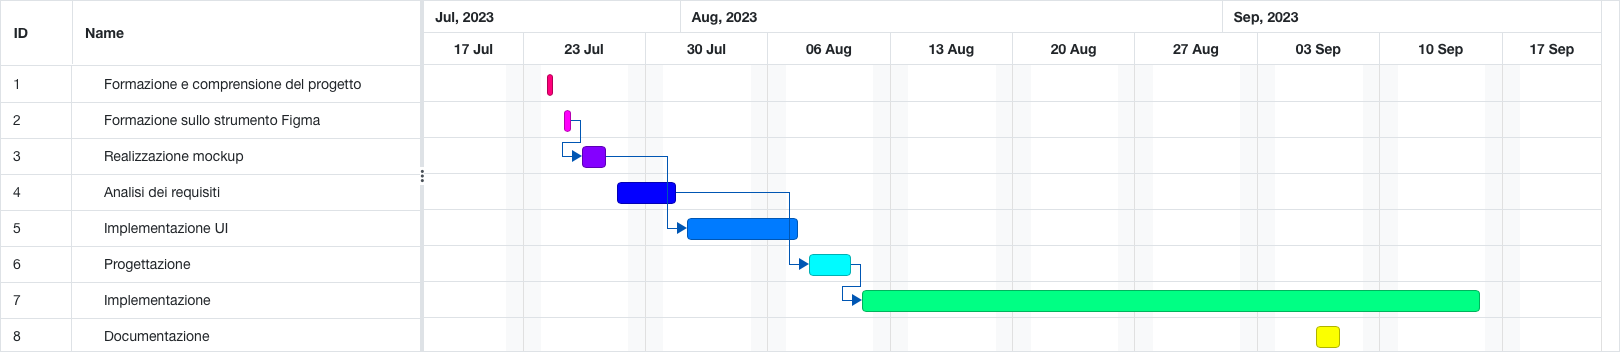
\includegraphics[width=1.0\columnwidth]{gantt_stage} 
    \caption{Diagramma di Gantt della ripartizione definitiva delle attività durante il periodo di stage}
    \label{fig:gantt}
\end{figure}

È doveroso precisare che, nonostante la fase di progettazione sia avvenuta dopo la codifica della \gls{uig}\glsoccur dell'applicazione e non vicerversa, come previsto nella pianificazione iniziale, ma soprattutto dai principi dell'\gls{ingsw}\glsoccur, non si è andati a compromettere la fase di sviluppo, in quanto la codifica della \gls{uig}\glsoccur si è svolta con la consapevolezza di implementare un'architettura che si basasse sul \gls{patternarchitetturale}\glsoccur \Gls{mvcg}\glsoccur, per mantenere una separazione tra la logica di presentazione e la logica di business.

\begin{table}
    \centering
    \begin{tabularx}{\textwidth}{|c|c|X|}
        \hline
        \textbf{Ore effettive} & \textbf{Ore pianificate} & \textbf{Descrizione dell'attività} \\\hline
        
        \textbf{70} & \textbf{80} & \textbf{Formazione sulle tecnologie} \\	 
        \hline
        
        \textbf{40} & \textbf{40} & \textbf{Definizione architettura di riferimento e relativa documentazione} \\ \hdashline 
        \multirow{3}{0cm}\\ 
        \textit{14} &
        \textit{12} & 
        \textit{Analisi del problema e del dominio applicativo} \\
        \textit{20} &
        \textit{22} & 
        \textit{Progettazione della piattaforma e relativi test} \\
        \textit{6} &
        \textit{6} & 
        \textit{Stesura documentazione relativa ad analisi e progettazione} \\
        \hline
        

        \textbf{192} & \textbf{160} & \textbf{Sviluppo}  \\ \hdashline 
        \multirow{5}{0cm}\\ 
        \textit{40} &
        \textit{26} & 
        \textit{Implementazione del meccanismo di autenticazione e integrazione con il sistema preesistente per il prelevamento dei dati da visualizzare nell'applicazione} \\
        \textit{40} &
        \textit{34} & 
        \textit{Implementazione delle funzionalità di creazione e compilazione (testuale e vocale) delle meeting-note} \\
        \textit{40} &
        \textit{28} & 
        \textit{Integrazione del servizio OpenAI} \\
        \textit{24} &
        \textit{40} & 
        \textit{Attività di testing} \\
        \textit{48} &
        \textit{32} & 
        \textit{Sviluppo UI} \\
        \hline
        
        \textbf{10} & \textbf{40} & \textbf{Verifica e Validazione finale}  \\ \hdashline 
        \multirow{3}{0cm}\\ 
        \textit{0} &
        \textit{24} & 
        \textit{Esecuzione dei test per la verifica e collaudo dell'applicazione} \\
        \textit{10} &
        \textit{8} & 
        \textit{Stesura documentazione finale} \\
        \textit{0} &
        \textit{8} & 
        \textit{Deploy dell'applicazione} \\
        \hline
        
        \textbf{312} & \multicolumn{2}{|c|}{\textbf{Totale ore}} \\ 
        \hline
        
    \end{tabularx}
    \caption{Consuntivo della durata delle attività}
    \label{tab:consultivo-ore}
\end{table}

\section{Valutazione personale}
\label{sec:valutazione-personale}

Il tirocinio è stato un'esperienza molto formativa, in quanto mi ha permesso di mettere in pratica le conoscenze e metodologie acquisite durante il percorso di studi in un contesto lavorativo.\\
Come già menzionato in precedenza, nonostante la mia familiarità con alcune delle tecnologie adottate, ho avuto modo di approfondirle e di imparare nuovi concetti, soprattutto per quanto riguarda il \emph{framework} \emph{Flutter}.\\
Inoltre, per la prima volta ho avuto modo di lavorare ad un progetto in maniera più professionale, seguendo anche alcuni principi affrontati durante il corso di \emph{Ingegneria del Software}, come ad esempio la pianificazione della fase di sviluppo, fissando delle \gls{milestone}\glsoccur, mantenendo traccia dei progressi per il raggiungimento degli obiettivi del progetto, e la documentazione del codice, in modo da rendere più facile la comprensione e la manutenzione del codice.\\  
L'azienda mi ha lasciato molta autonomia durante lo sviluppo del progetto e mi ha fornito un \emph{feedback} costante, permettendomi di migliorare e di imparare nuove cose. \\
In conclusione, ritengo che il tirocinio sia stato un'esperienza molto positiva, che mi ha permesso di crescere sia dal punto di vista professionale che personale. 